
\documentclass[12pt]{article}

\usepackage[utf8]{inputenc}
\usepackage[bulgarian]{babel}
\usepackage{graphicx}
\usepackage{sidecap}  %required for side captions
\usepackage{amssymb}
\usepackage{amsmath}
\usepackage{hyperref}
\usepackage{commath}  
\usepackage[top=1.3in, bottom=1.5in, left=1.3in, right=1.3in]{geometry}


\begin{document}
	\begin{center}
        \LARGE{\textbf{Тема: Разширение на проект от УЕБ: Система за записване и управление на присъствие по време на презентации, упражнения или лекции, посредством ползване на услугите AWS EC2 и AWS RDS}}
        
        \bigskip
        \Large{Предмет: AWS}
        
        \medskip
        \Large{Изготвил: Огнян Стоименов, фн: 81908, имейл: ostoimenov@uni-sofia.bg}
        
        \medskip
        \Large{Лектор: доц. д-р Милен Петров, година: 2022}
        
        \bigskip
	\end{center}
    
    
  %  \newpage
    \tableofcontents
    \bigskip
    \bigskip
    \newpage
  
\section{Условие} 
Системата за импортва списък със студенти ( с формат csv - от puffin, fn/email, от суси, фн, име,курс, група, специалност?), от БББ - текстов файл - на един ред , в името на файла е указан ден/час на направа на списъка, а във файла има по 1 присъстващ на ред); - Да се генерира по зададено събитие (да речем презентация) - с начало/край - колко пъти е проверявам някой и колко от проверките е присъствал; Да може да се прави статистика; през системата да се записва като присъствал (да речем през зададен ключ за занятие); да може да се 'обхождат' като в календар присъствията; За всеки присъствал занятие - да може да добавя коментар и да му се споделят ресурси от занятието; (например линкове, коментари, забележки, оценки); Ресурсите може да са линк на пдф на лекцията, инк за логване във видеото; линк със записа на лекцията (може всеки да ги добавя) - а инструктора одобрява кои да се виждат и кои не.

\section{Въведение}
Целта на проекта е да създаде малка и лесна система за следене на присъствията на студенти по време на лекциите. Лекциите са разделени на подлекции с цел следене на присъствие по време на различни дейности с различни интервали - пример представяне на реферати. Първата финална версия цели да позволи ползване на системата от преподаватели, но не и студенти към момента. 
\section{Теория}
\noindent За разширяването на Уеб приложението са използвани следните AWS услуги:  
\medskip

\noindent \textbf{AWS Relational Database Service (RDS):} услуга, която позволява лесно настройване, опериране и мащабиране на релационни бази данни като mysql, която се използва в разглеждания проект. AWS RDS се грижи за голяма част от административните задачи по поддържането на релационната база данни. Част от тези задачи са security updates, availability, data encryption, настройване на различни видове аларми и създаване на backup на базата. Има възможност за моментално интегриране на промени от потребителя (modify) или да се настрои период в който всички промени да влязат в сила едновременно. Това позволява на потребителя да се фокусира върху менажирането на съдържанието в базата.
\medskip

\noindent \textbf{AWS Elastic Compute Cloud (EC2):} уеб услуга, която осигурява сигурен, преоразмерим изчислителен капацитет в cloud-а чрез използване на виртуални машини. Този подход осигурява пълен контрол върху всички компютърни ресурси и позволява работа в сигурна среда на Amazon. Също така, предоставя лесна интеграция с други AWS услуги като например AWS RDS чрез Virtual Private Cloud (VPC), което е частна виртуална мрежа в cloud-а на Amazon.
\medskip

\section{Използвани технологии}
\noindent За изграждането на web приложението са използвани следните стандартни технологии и подходи:

\begin{itemize}
\item \textbf{Frond-end}: HTML5, CSS3, JavaScript
\item \textbf{Back-end}: PHP version 'PHP 8.1.6'
\item \textbf{Database}:  mysql Ver 8.0.27 for macos11 on x86\_64 (MySQL Community Server - GPL)
\item \textbf{Cloud}:
\begin{itemize}
\item AWS RDS
\item AWS EC2
\end{itemize}
\end{itemize}

%\newpage

\section{Инсталация и настройки}
\subsection{AWS Relational Database Service}
Създава се MySQ база данни с необходимата за проекта архитектура. Изпълняват се следните стъпки:
Свързването към базата \textbf{webproject} се осъществява с помощта на допълнителни инструменти като например MySQL client. В инструмента се въвежда endpoint и порт на използваната база. Предоставят се username и password, създадени при инициализацията на базата. Import-ва се .sql файл, който създава всички таблици със съответните ограничения и въвежда всички данни, налични до този момент в тях. След успешното изпълнение на стъпките, базата данни е готова за употреба.
\begin{figure}[!htb]
    \centering
        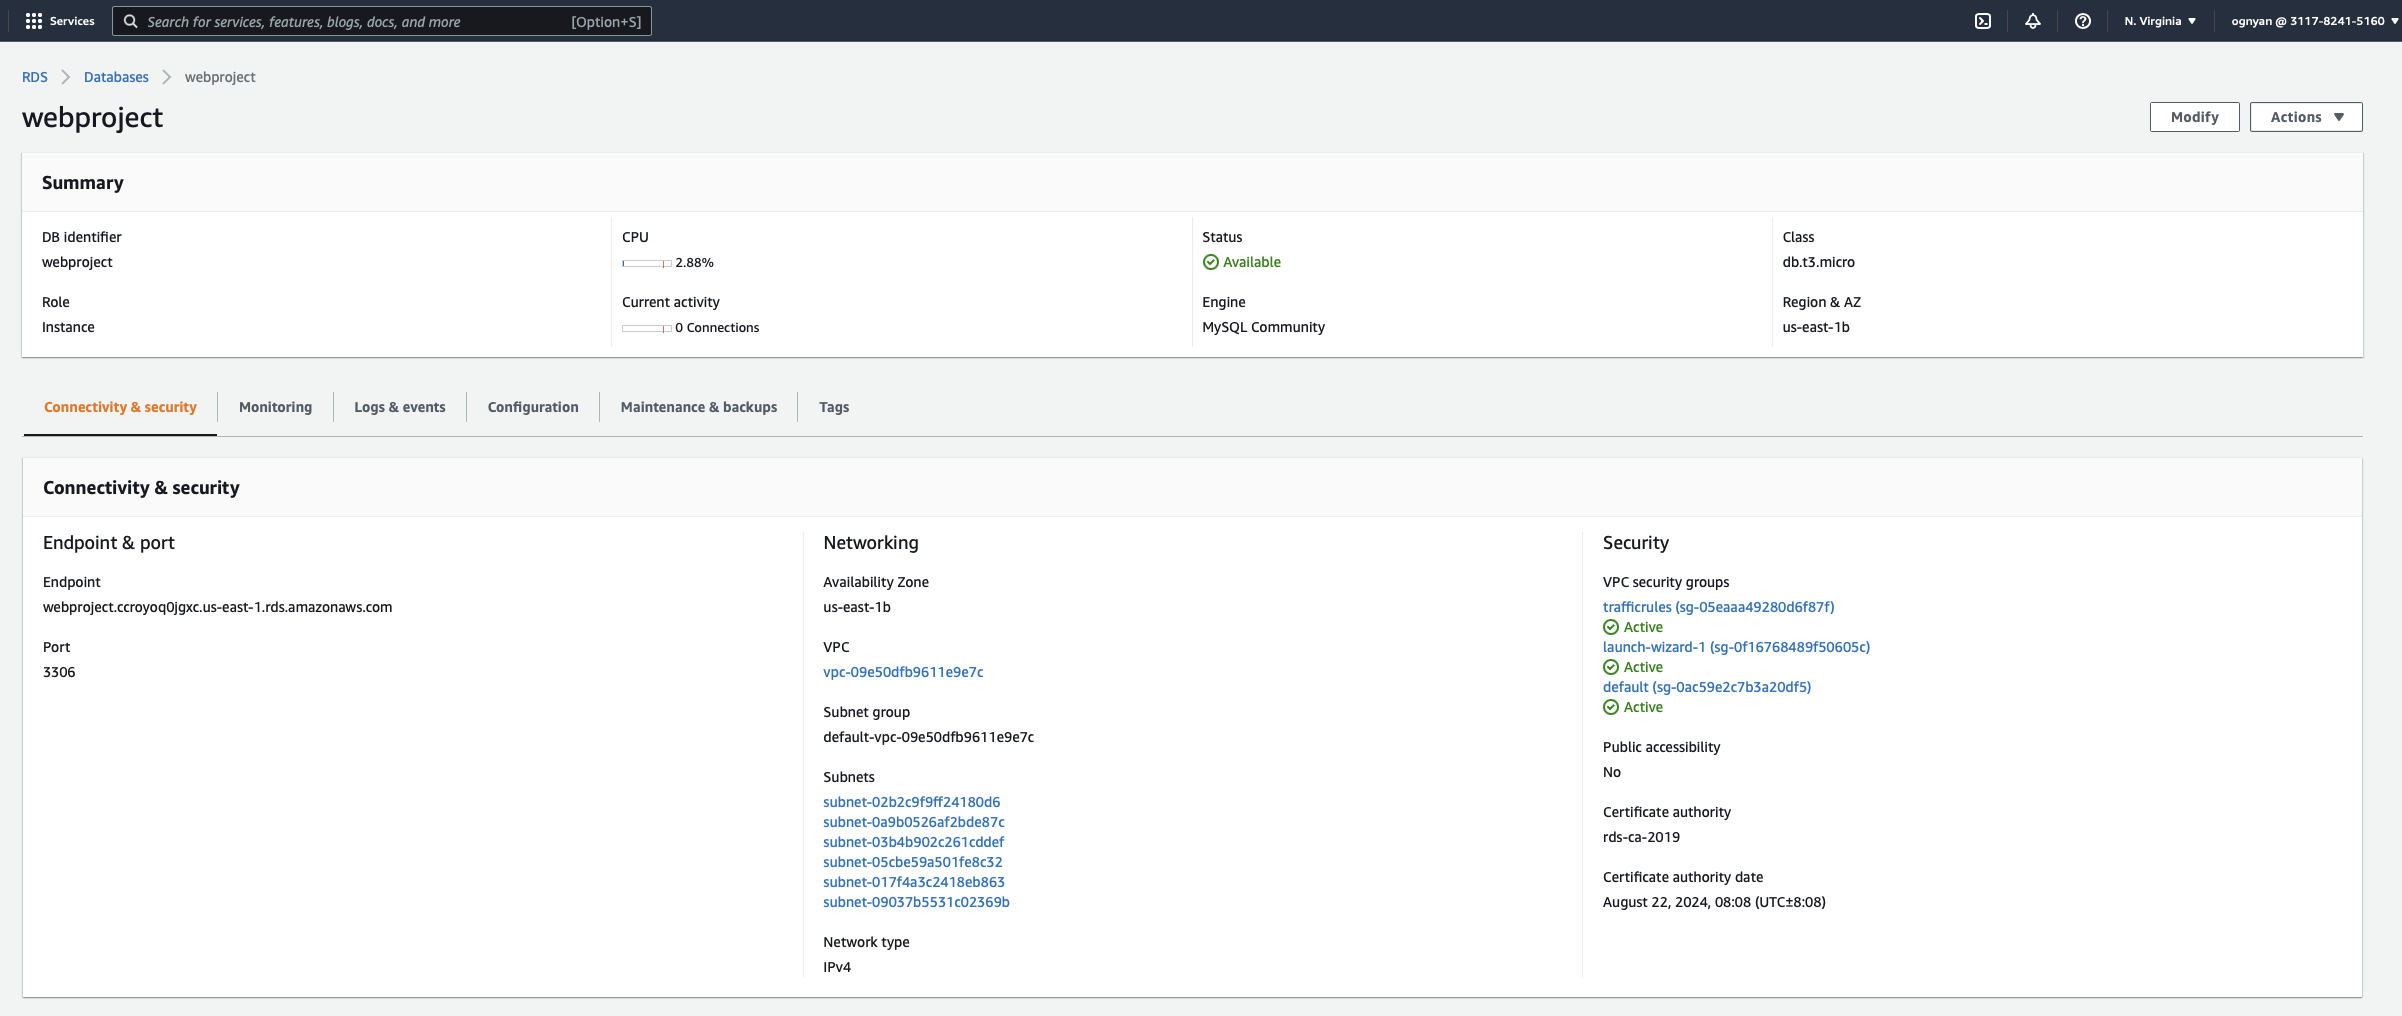
\includegraphics[scale=0.15]{81908_fig1.png}
    \caption{Настройки на базата \textbf{webproject} в AWS:}
\end{figure}
    
    \noindent  
    
Базата принадлежи на Security Group \textbf{trafficrules} 
\bigskip
\begin{figure}
\centering
        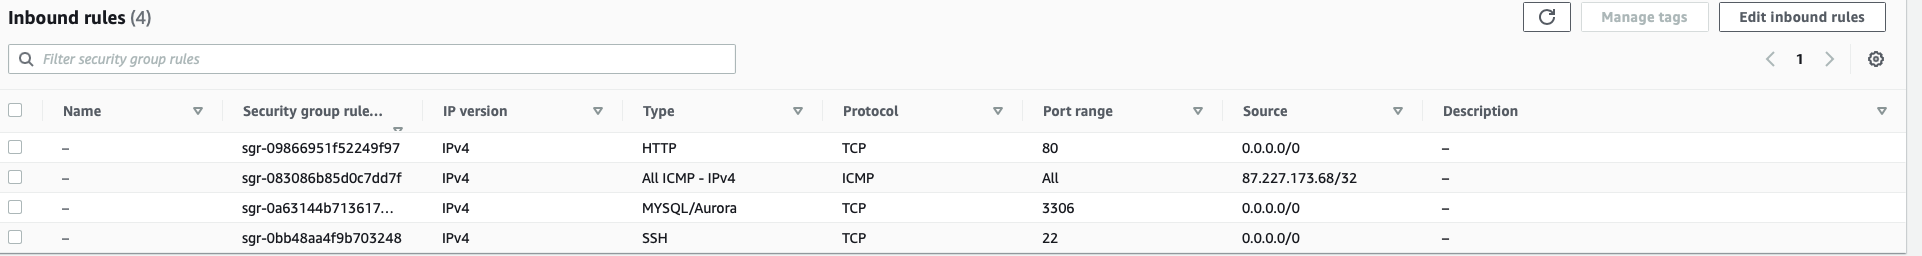
\includegraphics[scale=0.21]{81908_fig2.png}
        \caption{Настройки на \textbf{trafficrules}}
\end{figure}
\subsection{EC2}
Създаваме EC2 инстанция от aws console, като внимаваме да използваме само ресурси, достъпни за free tier. Също така за да комуникира с базата инстанцията трябва да е в същото VPC като базата! Тя също принадлеци на security групата \textbf{wepbroject}.

Като създадем инстанцията си запазваме ключа на машината, от която ще се свързваме.

Инсталираме apache, пускаме го и настройваме при всяко пускане на инстанцията, apache да се стартира автоматично :
\begin{figure}[h!]
    \centering
            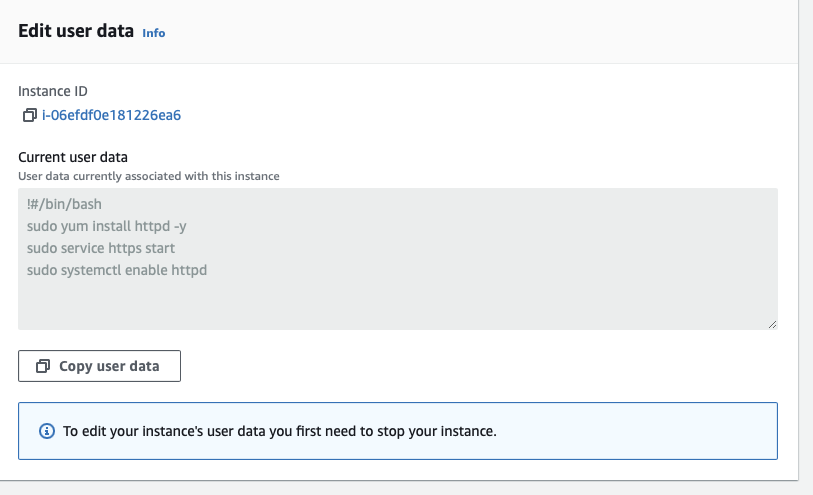
\includegraphics[scale=0.5]{81908_fig3.png}
            \caption{Настройки на EC2 -> user data}
    \end{figure}

Свързаме се с инстанцията или през aws уеб конзолата или чрез ssh: \\
> ssh -i ~/.ssh/macOS.pem ec2-user@ec2-54-91-67-180.compute-1.amazonaws.com

Инсталираме python версия ПОНЕ 8.0 на ec2: \\
> sudo  amazon-linux-extras enable php8.0 \\
> sudo yum install php8.0

Пулваме проекта в ec2 инстанцията:
> sudo yum install git \\
> git clone --single-branch --branch aws https://github.com/ognyanstoimenov/web-final-project.git \\

Слагаме проекта в дифолт директорията на apache:
> sudo mv -r web-final-project/ /var/www/http/

Настройваме apache да "сервира" само публик папката:
във файла /etc/httpd/conf/httpd.conf слагаме настройката \textbf{DocumentRoot /var/www/http/web-final-project/public}.

Приложнеието се достъпва от public IPv4 DNS на инстанцията.
Например пишем в браузъра:
ec2-54-91-67-180.compute-1.amazonaws.com

\pagebreak
\section{Кратко ръководство за потребителя}
\begin{figure}[!htb]
    \centering
            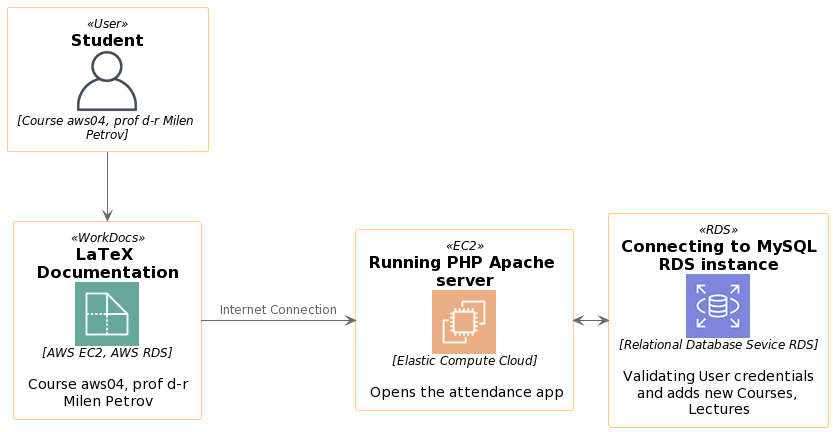
\includegraphics[scale=0.5]{81908_diagram.png}
            \caption{UML диаграма}
\end{figure}    
\section{Примерни данни}
Примерни данни качвани от потребителя от тип текстов файл. \\
List of users in meeting Лекция 27.10.2021г./всички лекции 9:15 (поток 1) и /11:15 (пото... at 12/15/2021:9:32:30 AM \\
Sorted by first name: \\
Габриела Бранкова \\
Георги Шавов \\
Георги Попов \\
Денислав Иванов \\
Димитър Ганев \\ 
Димитър Георгиев \\

\section{Описание на програмния код}

\subsection{Database}
Съдържа всички класове, които отговарят за връзката с базата. Базата се конфигурира от файла db.php и всички останали файлове ползват една инстанция на връзката с базата. Файловете предлагат интерфейс за работа с таблиците в базата, а в имплетементацията са конкретните SQL заявки.

\subsection{Models}
Моделите на уеб апликацията. Те се използват за лесно и удобно представяне на съответните модели от базата.
\subsection{Public}
Публичната част на апликацията - клиента. 
\subsection{Uploads}
Тук се съхраняват временно файловете, които потребителят качва докато бъдат обработени.
\medskip


\section{Приноси на студента, ограничения и възможности за бъдещо развитие}

Представената функционалност в този документ е изработена изцяло от автора на този документ. Възможности за бъдещо разширение:
Възможност студент да проверява присъствията си.
Опция преподавател да качва повече от един файл на един път.

\section{Какво научих}
Научих как да  създам цялостен уеб апп, качен в клауда. Научих се да боравя с aws конзолата. Научих как да използвам и комбинирам няколко aws services и как да ги конфигурирам. Научих как да боравя с бази данни използвайки PHP технологията,как да представя данни използвайки време като качество за сравнение с допълнителна библиотека.
\section{Списък с фигури и таблици}

\listoftables

\listoffigures

\section{Използвани източници}
\noindent\href{https://aws.amazon.com/ec2/}{[1] AWS Elastic Compute Cloud}

\noindent\href{https://aws.amazon.com/rds/}{[2] AWS Relational Database Service}

\noindent\href{https://learn.fmi.uni-sofia.bg/course/view.php?id=8205}{[3] Moodle Course FMI AWS 2022}

\noindent\href{https://awsacademy.instructure.com/courses/15407}{[4] AWS Academy Introduction to Cloud: Semester 2 [15407]}
\end{document}